%%% Thesis Introduction --------------------------------------------------
\chapter{Stochastic Cooperation}
\ifpdf
    \graphicspath{{StochasticCooperation/Figs/PNG/}{StochasticCooperation/Figs/PDF/}{StochasticCooperation/Figs/}}
\else
    \graphicspath{{StochasticCooperation/Figs/EPS/}{StochasticCooperation/Figs/}}
\fi
To simulate stochastic cooperation we use a more simple game where there are not pair interaction among individuals, this game is a system of common goods, where individuals in a group interact through a common source of any benefit.  This describes a classic game in behavioral economics\cite{Szabo2002} where a  group of people is given an amount of money, each person has to contribute money, and the total amount is divided by the number of people in the group, and then each individual gets back this quantity times a factor larger than one.

 In this model  each individual invests a random cost $c_{i}$, and everyone obtains a common benefit $b=B\frac{\sum c_{i}}{n}$, where the benefit factor $B\geqslant1$ . The utility of each individual is $u_{i}=b-c_{i}$. Therefore, if everyone cooperates with the same amount they get back a larger amount, but if just some individuals cooperate, they will get back a smaller amount than invested. Furthermore, if nobody cooperate, there will be not payoff. 
 
 The expected payoff of a cooperator is
   \begin{equation}
   \pi_{C}=\frac{\sum_{j=1}^{i}b-c_{cj}}{i}
   \end{equation}   
   and the fitness is
   \begin{equation}
   f_{c}=1-w+w\pi_{c}
   \end{equation} 
   In our simulations we used $w=1$.

 
    In a bacterial example, plasmids in E.coli are the individuals and the E.coli are the groups. The plasmids take nutrients from the cell for their own reproduction, but when they take too much the bacteria will reproduce slower. 
    Another example is when a group of bacteria produce  an enzyme to process a food source, which all the bacteria have equal accessibility.  
    
    
  We used this cooperation model to simulate group selection in individuals with no deterministic degree  of cooperation. The population was divided in two types, where their cooperation degrees come from Gaussian distributions with different means and standard deviations. Different measures of fixation probability as a function of noise and benefit were done for this system, as shown bellow.   
 \begin{figure}[H]
\begin{center}$
\begin{array}{cc}
a)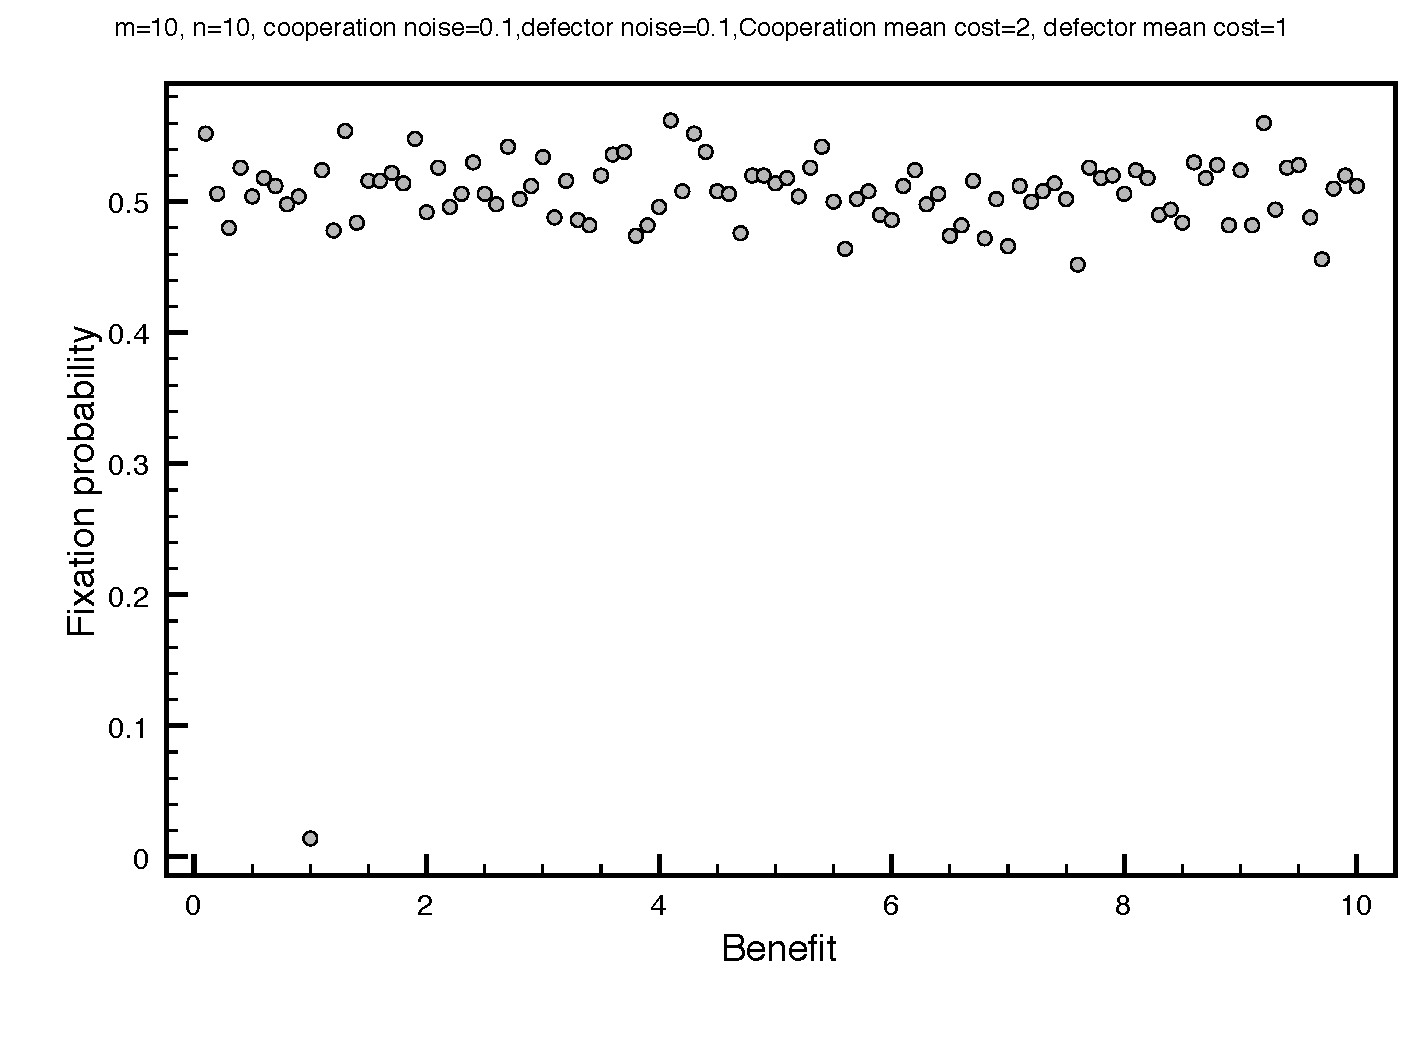
\includegraphics[width=2.5in]{fixprobabilityVsBenefit.pdf} &
b)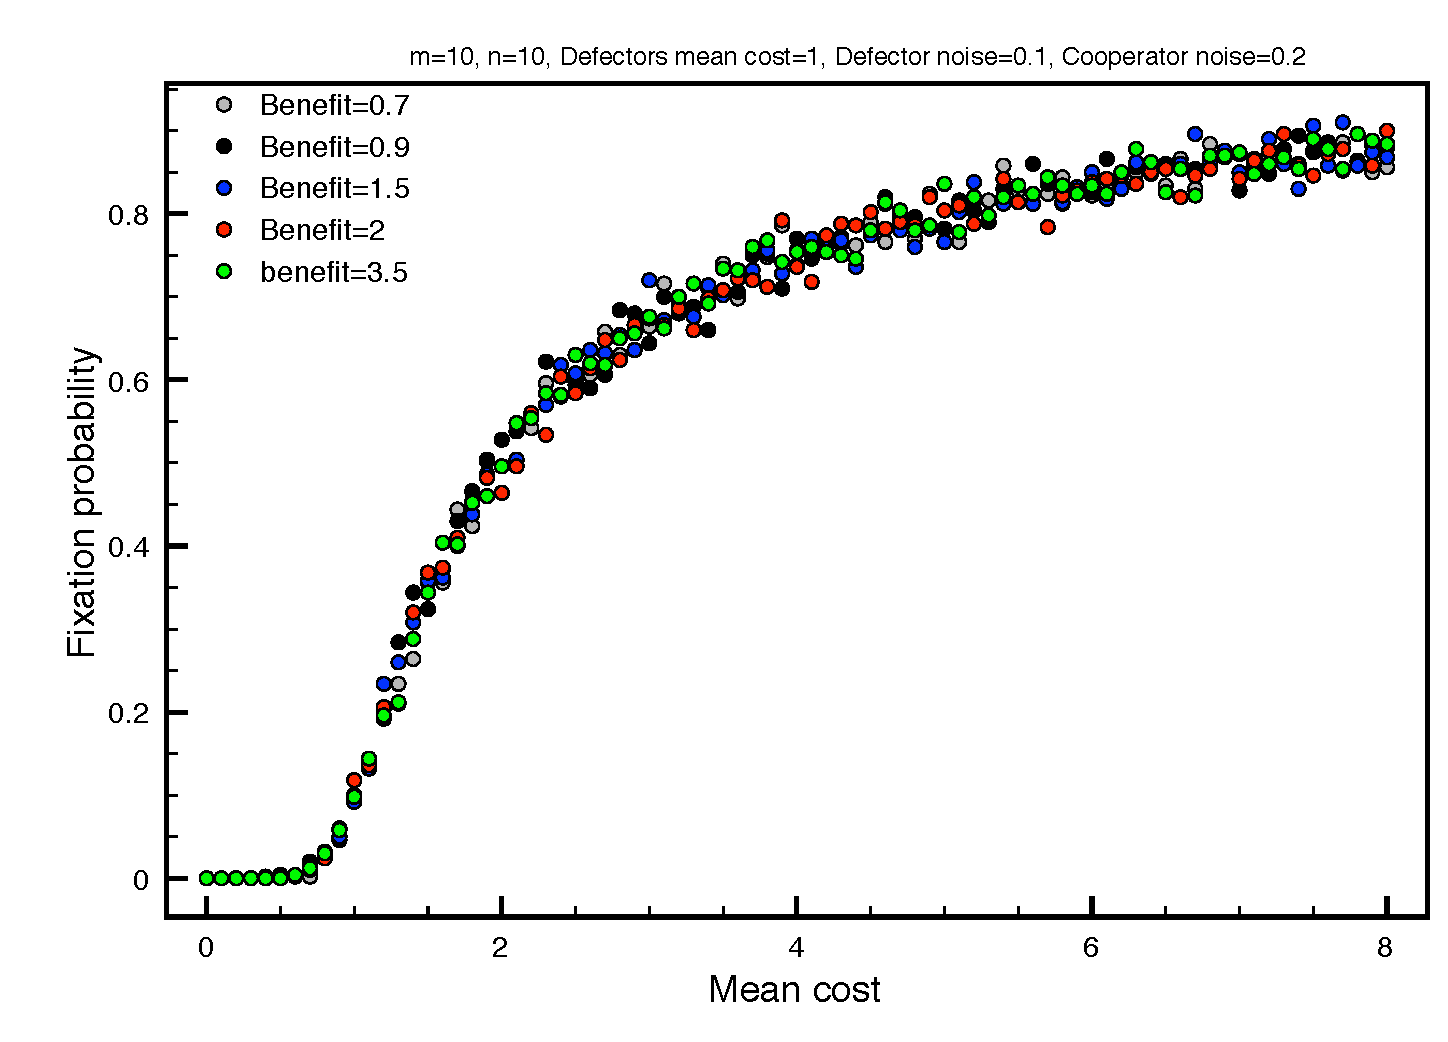
\includegraphics[width=2.7in]{fixprobabilityVsmean1Benefit.pdf}
\end{array}$
\end{center}
\caption{a): Fixation probability as a function of benefit when initially all groups are homogeneous . b): Fixation probability as a function of mean cost for several values of benefit.}
\label{Fig8.1}
\end{figure}

\begin{figure}[H]
\begin{center}$
\begin{array}{cc}
a)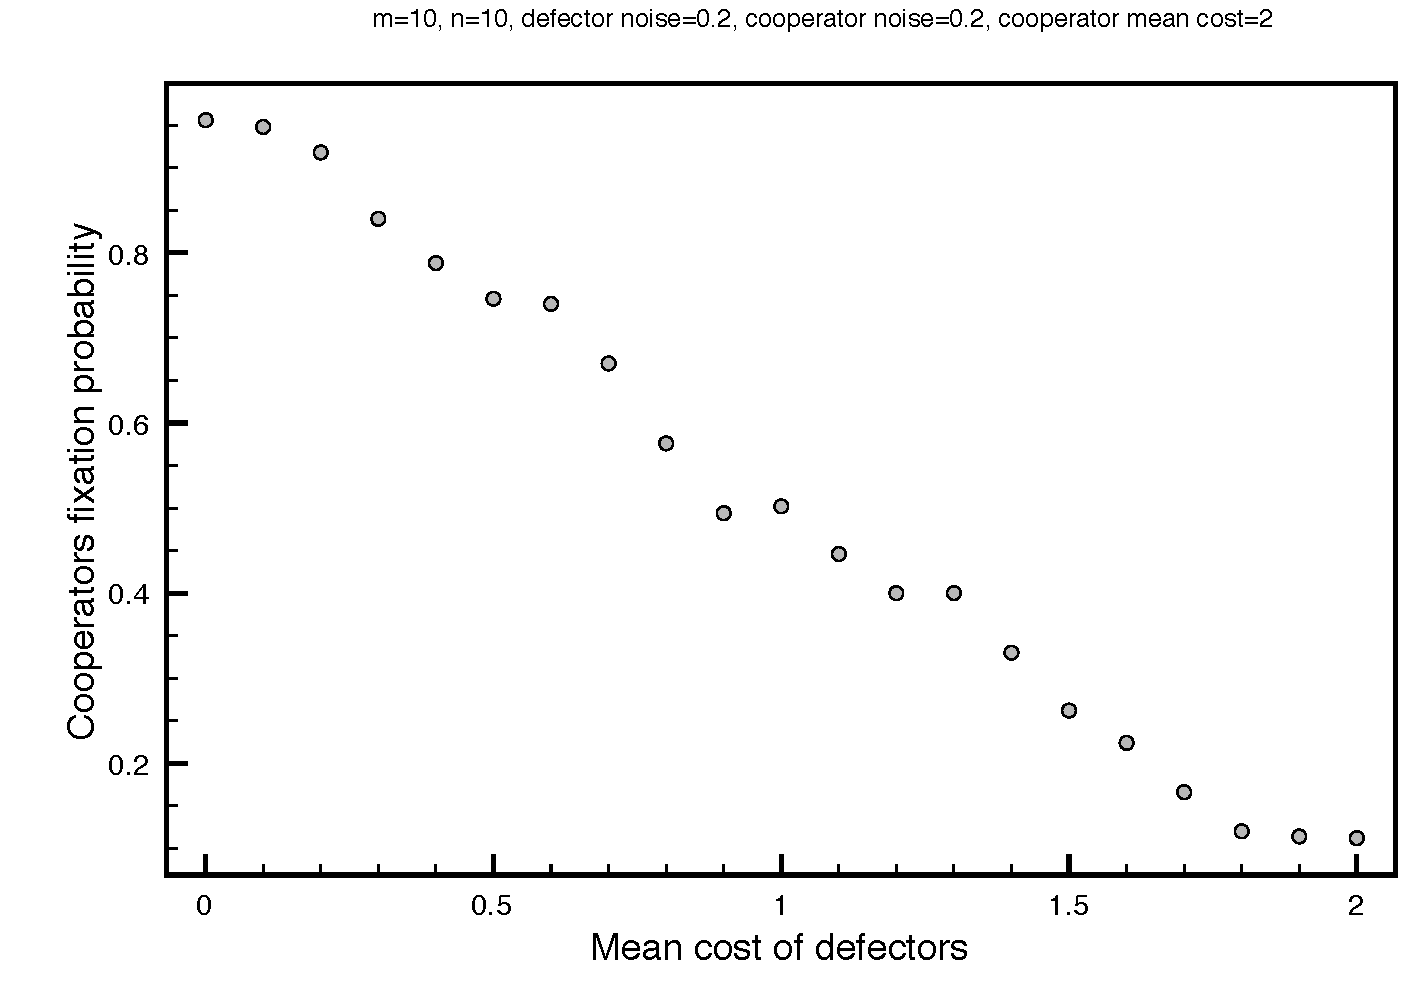
\includegraphics[width=2.5in]{fixprobabilityVsmean0.pdf} &
b)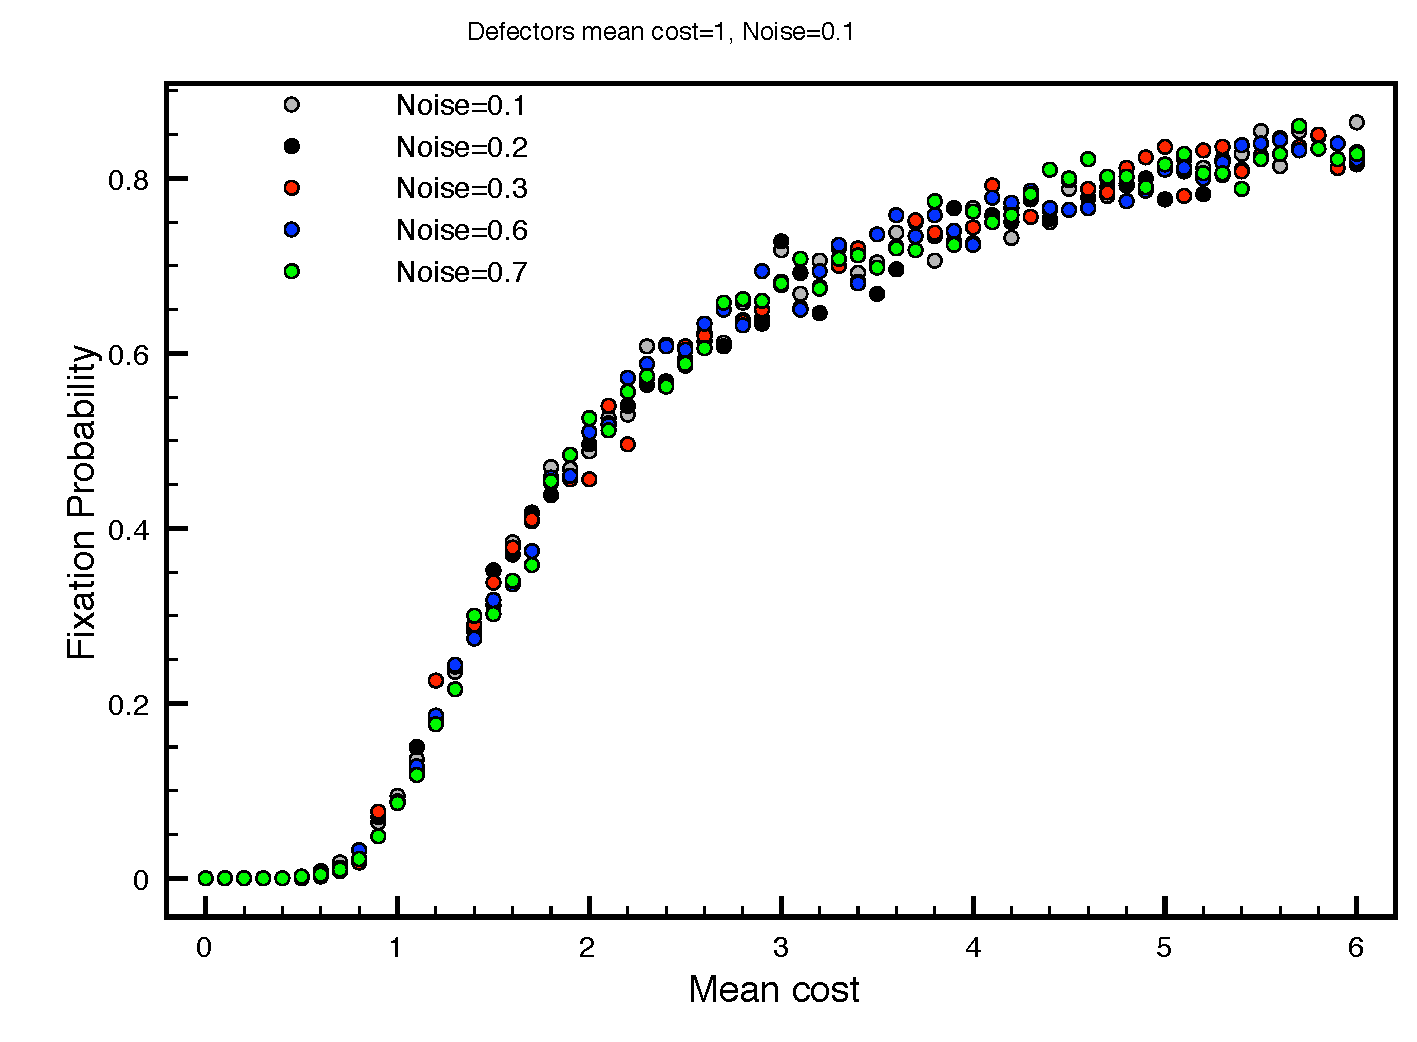
\includegraphics[width=2.7in]{fixprobabilityVsmean1Sigmas.pdf}
\end{array}$
\end{center}
\caption{a): Fixation probability of cooperators as a function of mean degree of defectors cooperation. b): Fixation probability of cooperators as a function of their mean degree cost. The graph shows different points for several values of benefit when all the groups are initially homogeneous.}
\label{Fig8.2}
\end{figure}
It  is seen that initially for a group where there is a defector, this individual have a larger probability of reproduction than the rest of the group, but as this kind of individuals reproduce, the overall fitness of the group decreases respect to the rest of the groups with cooperators.
\begin{figure}[H]
\begin{center}$
\begin{array}{cc}
a)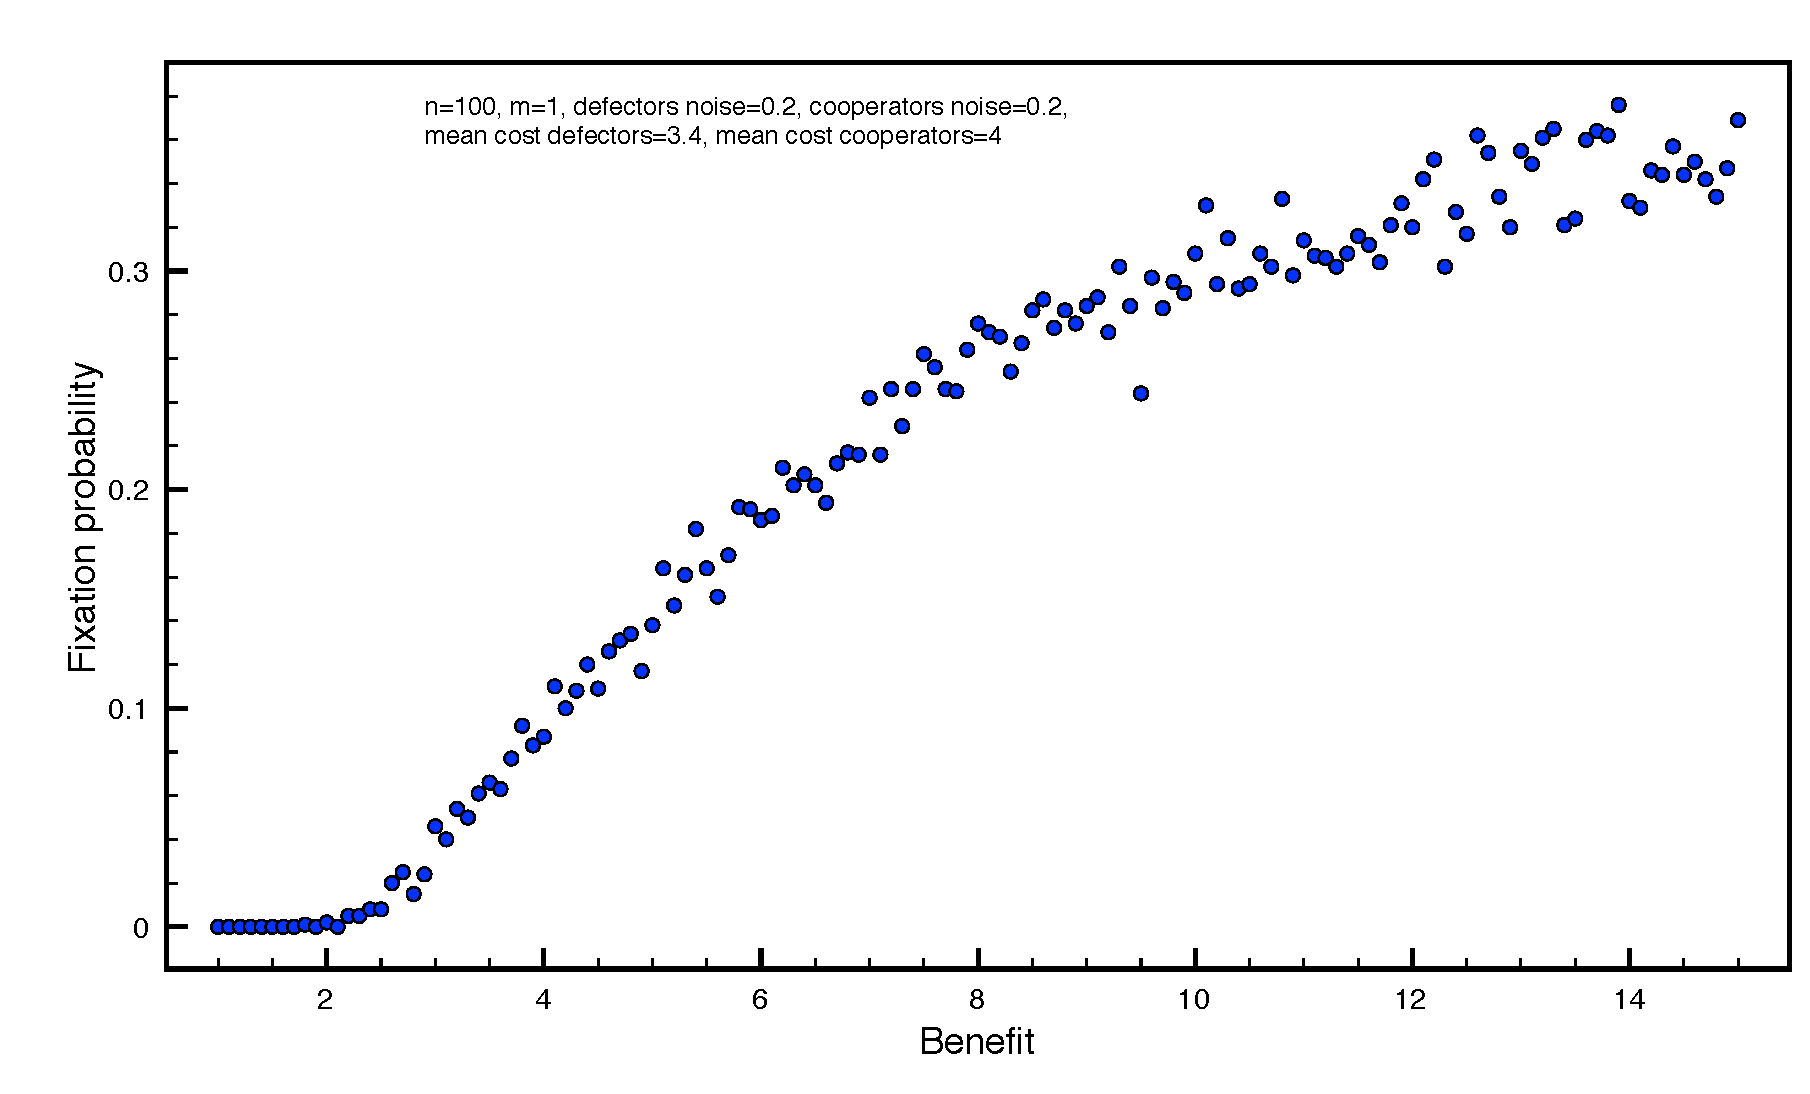
\includegraphics[width=2.5in]{probaCoopeSinglegroup.pdf} &
b)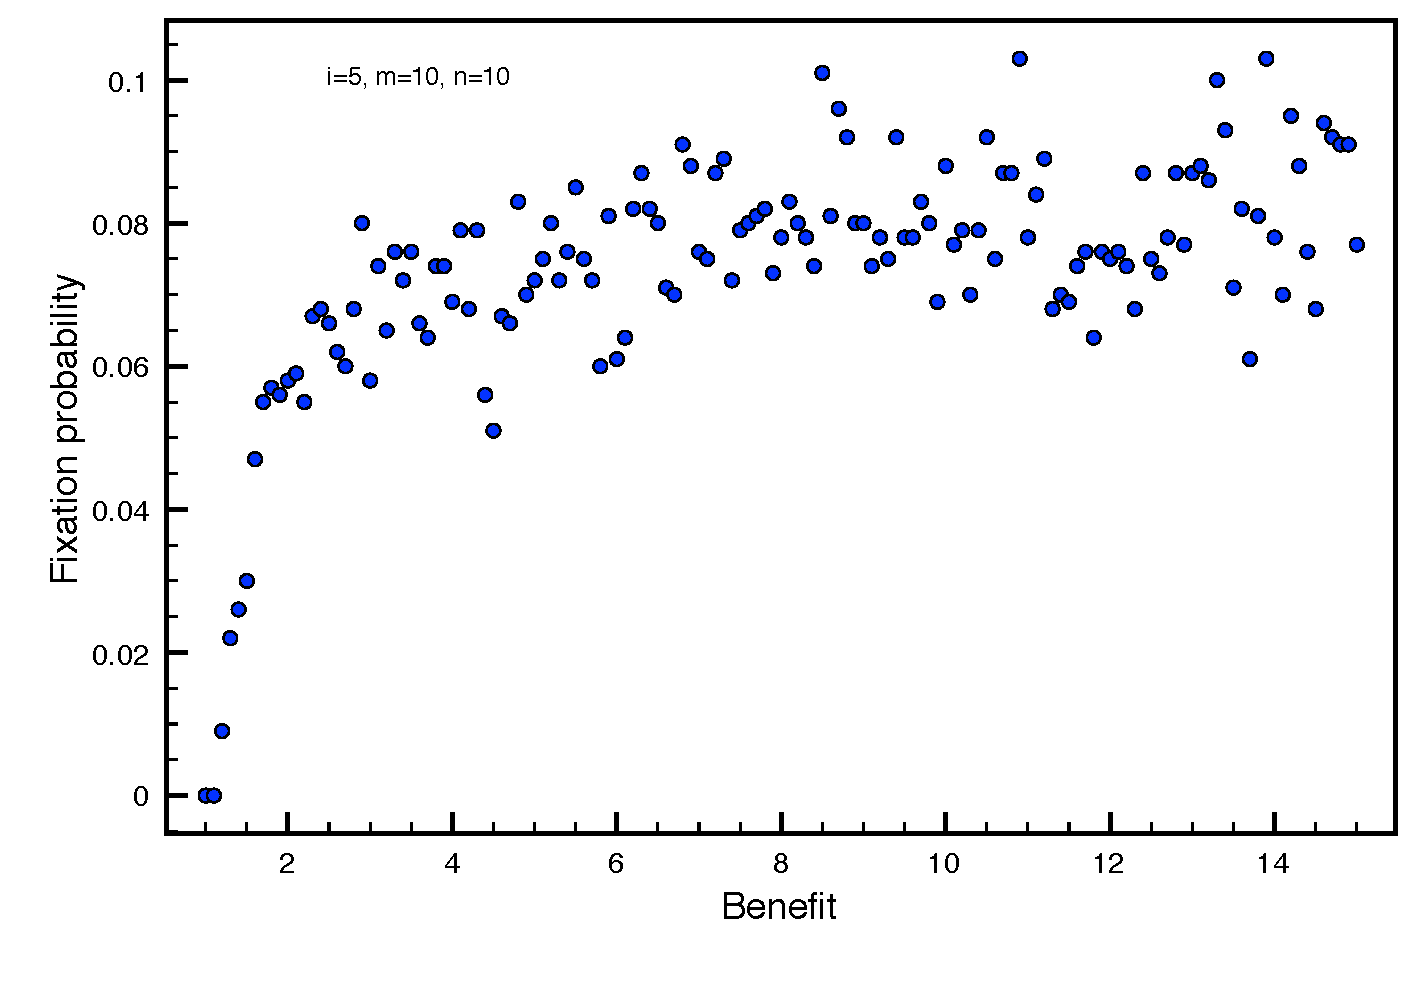
\includegraphics[width=2.7in]{probaCoomixedGroup.pdf}
\end{array}$
\end{center}
\caption{a): Fixation probability of $50$ cooperators in a group of size $100$. b): Fixation probability when a population of $m=10$ and $n=10$ has initially a mixed group with $5$ cooperators and the rest of the groups are deffectors.}
\label{Fig8.3}
\end{figure}

%%% ----------------------------------------------------------------------

%%% Local Variables: 
%%% mode: latex
%%% TeX-master: "../thesis"
%%% End: 
